%!TEX root = ../toolhinweise.tex

\section{Installation und Konfiguration}
\label{sec:installation}


\textbf{YAKINDU Statechart Tools (SCT)} ist ein Eclipse-Plugin.
Da es gelegentlich zu Problemen mit einem nachinstallierten Plugin kommt, empfehlen wir YAKINDU SCT als separates Standalone-Programm zu installieren. 

Für die Kombination von YAKINDU SCT mit dem für das \docProjectTitle{} gegebenen Validierungsframework wird ein \textbf{Java Development Kit (JDK)} mit \textbf{mindestens Version 10} benötigt (getestet mit den Versionen 10.0.2, 11.0.2, 12.0.1 und 17.0.2 LTS und 18.0.1.1). In dieser Installationsanleitung wird die neuste Version Java 18.0.1.1 verwendet und YAKINDU SCT 4.0.





%%%%%%%%%%%%%%%%%%%%%%%%%%%%%%%%%%%%%%%%%%%%%%%%%%%%%%%%%%%%%%%%%%%%%%%%%%%%%%%%%%%%%%%%%%%%%%%%%%%%%%%%%%%%%%%%%%%





\subsection{JDK und YAKINDU SCT installieren}

\subsubsection{Windows 10}

\begin{enumerate}
	\setlength\topsep{-1em}
	\setlength\itemsep{-0.5em}
	\item Java herunterladen (auf der Webseite die .exe-Datei auswählen):
	\\\url{https://www.oracle.com/java/technologies/downloads/#jdk18-windows}
	\item Java gemäß den Anweisungen installieren.
	\item Falls noch nicht automatisch erfolgt, Java zur System-Path-Variable hinzufügen:
	\vspace{-0.5em}
	\begin{enumerate}
		\setlength\itemsep{-0.5em}
		\item In der Suchleiste \enquote{Systemumgebungsvariablen bearbeiten} suchen und öffnen.
		\item Den Button \enquote{Umgebungsvariablen} anklicken. 
		\item Die Variable \enquote{Path} im unteren Bereich \enquote{Systemvariablen} auswählen und \enquote{Bearbeiten} klicken. 
		\item Falls Java noch nicht eingetragen ist, hier den Pfad der neuen Java-Installation hinzufügen (z.B. \texttt{C:\textbackslash{}Program Files\textbackslash{}Java\textbackslash{}jdk-17.0.2\textbackslash{}bin}).
	\end{enumerate}
	\item YAKINDU Statechart Tools Professional für \enquote{Windows 64 Bit} Edition herunterladen:
	\\\url{https://www.itemis.com/en/yakindu/state-machine/download-options/}
	\item Heruntergeladene .zip-Datei an einem beliebigen Ort entpacken.
	\item Nachdem die .zip-Datei entpackt wurde, im entpackten Ordner die Datei \texttt{SCT.exe} ausführen.
\end{enumerate}

\subsubsection{MacOS X}

\begin{enumerate}
	\setlength\topsep{-1em}
	\setlength\itemsep{-0.5em}
	\item Java herunterladen (auf der Webseite die .dmg-Datei für die entsprechende Architektur auswählen):
	\\\url{https://www.oracle.com/java/technologies/downloads/#jdk18-mac}
	\item Java gemäß den Anweisungen installieren.
	\item YAKINDU Statechart Tools Professional für \enquote{macOS X 64 Bit} Edition herunterladen:
	\\\url{https://www.itemis.com/en/yakindu/state-machine/download-options/}
	\item Heruntergeladene \texttt{YAKINDU SCTPRO.app} in den Ordner Programme verschieben und starten.
\end{enumerate}



\subsubsection{Linux}

Die Installation auf Linux wurde mit Ubuntu Versionen 18.10, 19.04 und 20.04 getestet. Bei anderen Distributionen ergeben sich ggf. Abweichungen.


\subsubsection*{Variante 1: JDK über PPA beziehen}
\begin{enumerate}
	\setlength\topsep{-1em}
	\setlength\itemsep{-0.5em}
	\item \texttt{sudo add-apt-repository ppa:linuxuprising/java}
	\item \texttt{sudo apt-get update}
	\item \texttt{sudo apt-get install oracle-java18-installer}
	\item Falls mehrere Java-Versionen installiert sind: \\\texttt{sudo apt-get install oracle-java18-set-default}
	\item Installation mit \texttt{javac -version} prüfen.
\end{enumerate}



\subsubsection*{Variante 2: JDK direkt herunterladen}
\begin{enumerate}
	\setlength\topsep{-1em}
	\setlength\itemsep{-0.5em}
	\item Java herunterladen:
	\\\url{https://www.oracle.com/java/technologies/downloads/#jdk18-linux}
	\item Zur manuellen Java-Installation von Java aus einer .tar.gz-Datei diese entpacken und den Anweisungen der beiliegenden \texttt{README}-Datei folgen.
\end{enumerate}


\subsubsection*{Beide Varianten: YAKINDU SCT installieren}
\begin{enumerate}
	\setlength\topsep{-1em}
	\setlength\itemsep{-0.5em}
	\item YAKINDU Statechart Tools Professional für \enquote{Linux 64 Bit} Edition herunterladen:
	\\\url{https://www.itemis.com/en/yakindu/state-machine/download-options/}
	\item Heruntergeladene .zip-Datei an einem beliebigen Ort entpacken.
	\item Nachdem die .zip-Datei entpackt wurde, im entpackten Ordner die Datei \enquote{\texttt{SCT}} als ausführbar markieren und starten.
\end{enumerate}




%%%%%%%%%%%%%%%%%%%%%%%%%%%%%%%%%%%%%%%%%%%%%%%%%%%%%%%%%%%%%%%%%%%%%%%%%%%%%%%%%%%%%%%%%%%%%%%%%%%%%%%%%%%%%%%%%%%




\subsection{YAKINDU SCT aktivieren}

Für Mitarbeiter und Studierende des Hasso-Plattner-Instituts steht eine akademische Lizenz für die Professional Edition von YAKINDU SCT zur Verfügung.
Für die Bearbeitungsdauer vom \docProjectTitle{} genügt unter Umständen aber auch die automatisch vorinstallierte 30-Tage Probelizenz.



\subsubsection*{Akademischen Lizenz beantragten}

Auf der folgenden Webseite kann mit Angabe einer Universitäts-Email-Adresse eine kostenlose akademische Lizenz beantragt werden:

\begin{center}
	\url{https://www.itemis.com/en/yakindu/state-machine/licenses#professional-edition-academic-license}
\end{center}


In der Regel dauert es 1 Tag bis zur Freigabe. Es kann nach Ablauf der Lizenz mit der selben Email-Adresse eine neue beantragt werden.



\subsubsection*{Einbinden der akademischen Lizenz}

\begin{enumerate}
	\setlength\topsep{-1em}
	\setlength\itemsep{-0.5em}
	\item YAKINDU SCT zeigt zuerst einen \enquote{Welcome Screen} an. Diesen schließen.
	\item Im Menü unter \enquote{Window} das Fenster \enquote{Preferences} öffnen.
	\item Dort \enquote{YAKINDU Licences} (vorletzter Punkt) auswählen.
	\item Auf \enquote{Import License File...} klicken.
	\item Die per E-Mail erhaltene Datei auswählen.
	\item Bestätigen und das Einstellungsfenster schließen.
\end{enumerate}





%%%%%%%%%%%%%%%%%%%%%%%%%%%%%%%%%%%%%%%%%%%%%%%%%%%%%%%%%%%%%%%%%%%%%%%%%%%%%%%%%%%%%%%%%%%%%%%%%%%%%%%%%%%%%%%%%%%





\subsection{\enquote{\red{PROJEKTNAME}}-Projekt einrichten}
\label{subsec:import}

\subsubsection{Projektdaten beziehen}

Das \enquote{\red{PROJEKTNAME}}-Projekt wird über \red{HIER LINK ZUM REPOSITORY} bereitgestellt.
Es wird empfohlen das Repository zu forken, um stets aktuelle Updates zu erhalten.
In dem Repository können zudem Issues gemeldet werden.

% Der aktuelle Stand des Repositories wird zudem als .zip-Archiv im Moodle bereitgestellt.


\subsubsection{\enquote{\red{PROJEKTNAME}}-Projekt in YAKINDU SCT importieren}


Das Repository beinhaltet einen Eclipse-Projektordner, der in YAKINDU SCT importiert werden kann.

\begin{enumerate}
	\setlength\topsep{-1em}
	\setlength\itemsep{-0.5em}
	\item Den Projektordner (über das Repository oder die .zip-Datei im Moodle) auf der Festplatte speichern.
	\item YAKINDU SCT, wie oben beschrieben, starten und den \enquote{Welcome Screen} schließen.
	\item Links im \enquote{Project Explorer} einen Rechtsklick machen und \enquote{Import} auswählen.
	\item Dort \enquote{General} $\rightarrow$ \enquote{Existing Projects into Workspace} auswählen.
	\item Dann oben rechts auf \enquote{Directory} klicken und Projektordner auswählen.
	\item In der Projektliste sollte ein Projekt mit dem Namen \enquote{mod2-2022-sctsim} angezeigt werden. Dieses auswählen.
	\item Auf \enquote{Finish} klicken, um den Import abzuschließen. Das Projekt ist jetzt links im \enquote{Project Explorer} verfügbar.
\end{enumerate}



\subsection{Problembehebung}

Das vorgegebene Eclipse-Projekt enthält alle notwendigen Einstellungen und sollte in den meisten Fällen direkt benutzbar sein.

Es kann allerdings passieren, dass lokale Einstellungen (z.B. die installierte Java-Version) Teile der Projektkonfiguration überschreiben. In diesem Fall können die relevanten Einstellungen manuell geändert werden.
Dies ist auch notwendig, wenn, anstatt ein Projekt zu importieren (wie im \autoref{subsec:import} beschrieben), ein neues Eclipse-Projekt angelegt wird.

Zum Anpassen der Projekteinstellungen kann im \enquote{Project Explorer} das \enquote{mod2-2022-sctsim}-Projekt mit einem Rechtsklick angeklickt und \enquote{Properties} ausgewählt werden.

\enlargethispage{1\baselineskip}

\subsubsection{Java-Version manuell festlegen} 

Ist keine oder eine falsche Version von Java eingebunden, kann dies in den Projekteinstellungen geändert werden.


\begin{figure}
	\centering
	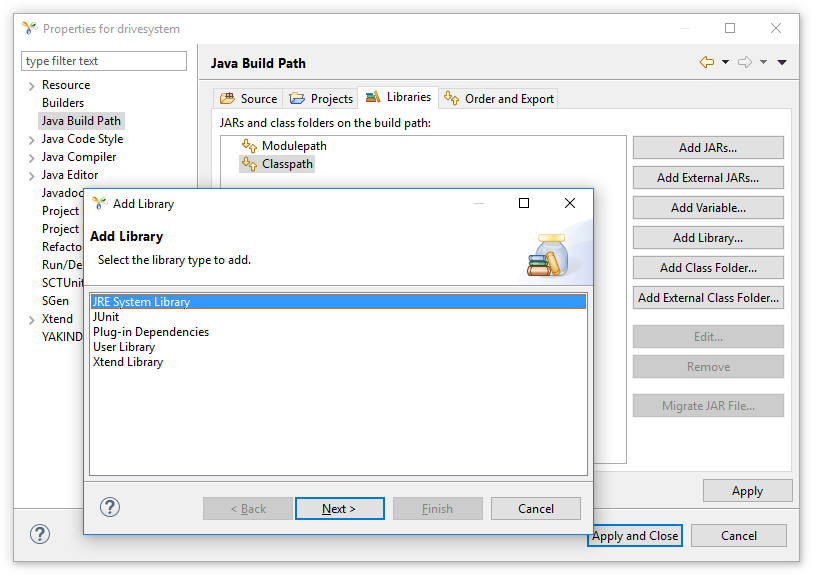
\includegraphics[width=0.7\textwidth]{yakindu_java_version}
	\caption{In den Projekteinstellungen kann eine bestimmte JRE-Version festgelegt werden}
	\label{fig:yakindu_java}
\end{figure}

In den Einstellungen wird dazu \enquote{Java Build Path} ausgewählt und dort der Tab \enquote{Libraries} geöffnet. Mit dem Button \enquote{Add Library...} kann eine \enquote{JRE System Library} hinzugefügt werden (siehe \autoref{fig:yakindu_java}).
Falls in der Liste bereits ein JRE-Eintrag vorkommt, kann dieser per \enquote{Edit...} angepasst werden. 
Mit einem Klick auf \enquote{Installed JREs...} kann die Liste der Eclipse bekannten Java-Versionen eingesehen und bearbeitet werden.

In manchen Fällen muss neben dem JRE-Eintrag auch noch ein JUnit-Eintrag hinzugefügt werden. 
Dabei muss JUnit Version 4 ausgewählt werden.

In seltenen Fällen wird nach dem Ändern der Java-Version an einigen Stellen im Code das Keyword \texttt{var} weiterhin als Fehler erkannt. 
Um dies zu vermeiden, bietet Eclipse als Korrekturvorschlag an, die \enquote{Project compliance} auf die neue Java-Version zu setzen. 
Zum Nutzen eines Korrekturvorschlags kann auf eine der Fehlermeldungen im \enquote{Problems}-Fenster oder an der entsprechend markierten Stelle im Code rechts geklickt werden.




\subsubsection{Projektordner manuell festlegen}

Wenn beim Programmstart Dateien nicht gefunden werden können, könnte es sinnvoll sein, die Liste der eingebundenen Quelltextordner in den Projekteinstellungen zu kontrollieren.


\begin{figure}
	\centering
	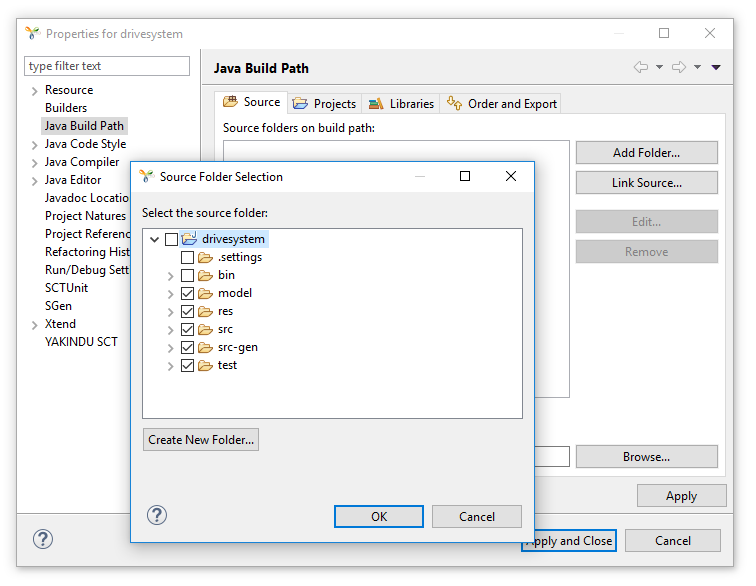
\includegraphics[width=0.7\textwidth]{yakindu_folders}
	\caption{In den Projekteinstellungen können die vom Eclipse-Projekt eingebundenen Quelltextordner festgelegt werden}
	\label{fig:yakindu_folders}
\end{figure}

Dazu wird in den Einstellungen der \enquote{Java Build Path} ausgewählt und dort der Tab \enquote{Source} geöffnet. 
Mit dem Button \enquote{Add Folder...} können nun Ordner hinzugefügt werden  (siehe \autoref{fig:yakindu_folders}).
Es müssen die Ordner \texttt{model}, \texttt{res}, \texttt{src}, \texttt{src-gen} und \texttt{test} ausgewählt werden.

\enlargethispage{1\baselineskip}


\subsubsection{Eclipse-Projekt umbenennen} 

In seltenen Fällen vergibt YAKINDU SCT dem \enquote{mod2-2022-sctsim}-Projekt beim Importieren einen anderen Namen (wie z.B. \enquote{mod2-2022-sctsim-master}).
In diesen Fällen muss das importierte Projekt umbenannt werden, da für die Codegenerierung der Projektname unbedingt \enquote{mod2-2022-sctsim} lauten muss. 
Zum Umbenennen muss im \enquote{Project Explorer} rechts auf das Projekt geklickt werden und \enquote{Refactor} $\rightarrow$ \enquote{Rename} ausgewählt werden.

